\documentclass[a4paper, 10pt, twocolumn]{article}

\NeedsTeXFormat{LaTeX2e}

%---------------------------- PACKAGE INCLUSION -------------------------------
% This group renders characters clearer and more precise

\RequirePackage[bitstream-charter,cal,expert]{mathdesign}
\RequirePackage{latexsym}

\usepackage{geometry} % to change the page dimensions
\geometry{a4paper,
		  %showframe=true,
		  %margin=3em,
		  %a4paper,
		  %total={170mm,257mm},
		  top=4.15em,
		  left=3em,
		  right=3em,
		  bottom=3.39em
		  }
		  
\usepackage[default]{cantarell}
\usepackage{xspace}
\usepackage{paralist}
\usepackage[parfill]{parskip} % Activate to begin paragraphs with an empty line rather than an indent
\usepackage{graphicx} % support the \includegraphics command and options
\usepackage{verbatim}
\usepackage{epsfig}
\usepackage{booktabs}

\newcommand{\phdcandidate}{Ph.D.~(ABD)\xspace}

\newcommand{\diplinfn}{Dipl.--Inf.\xspace}

\newcommand{\pos}{ERP~software--system\xspace}

\newcommand{\yerenlabs}{\textsc{YEROTH~R\&D}\xspace}

\newcommand{\yerenpos}{\textcolor{yerenColorBlue}{\sc YEROTH--ERP--$3.0$}\xspace}

\newcommand{\myfullacademicname}{Xavier NOUMBISSI NOUNDOU,~Dipl.--Inf.,~Ph.D.~(ABD)\xspace}

\usepackage{hyperref}
\hypersetup{
    colorlinks,
	pagebackref,
    citecolor=medgreen,
    linkcolor=purplish,
    breaklinks,
    pdftex,
    bookmarks,
    plainpages=false,
	pdftitle={Information Brochure of the \pos \yerenpos by: ''\myfullacademicname''},
    pdfauthor={Xavier NOUMBISSI NOUNDOU}
}

\usepackage{url}

\usepackage{xcolor}
\definecolor{yerenColorOrange}{RGB}{242, 161, 0}   
\definecolor{yerenColorBlue}{RGB}{77 , 93 , 254}
\definecolor{yerenColorRed}{RGB}{254, 48 , 48}
\definecolor{yerenColorDarkgray}{RGB}{60, 60 , 60}
\definecolor{yerenColorIndigo}{RGB}{83, 0, 125}
\definecolor{yerenColorGreen}{RGB}{2  , 160, 70}
\definecolor{forestgreen}{RGB}{2,160,70}    
\definecolor{mediumblue}{RGB}{7,43,205}    
\definecolor{firebrickred}{RGB}{178,34,34}
\definecolor{listingray}{gray}{0.9}
\definecolor{lbcolor}{rgb}{0.9,0.9,0.9}
\definecolor{darkgreen}{rgb}{0,0.35,0}
\definecolor{medgreen}{rgb}{0,0.5,0}
\definecolor{lightgreen}{rgb}{0.5,0.7,0.5}
\definecolor{pmcolour}{rgb}{0.5,0.7,0.5}
\definecolor{medgrey}{rgb}{0.6,0.6,0.6}
\definecolor{purplish}{rgb}{0.4,0,0.6}
\definecolor{brightred}{rgb}{1,0.2,0.2}

\newcommand{\yeren}{\textsc{yeroth--erp--3.0}\xspace}

\newcommand{\all}{<< CMUP >>\xspace}
\newcommand{\defdeo}{<< DEF\_DEO >>\xspace}
\newcommand{\fifo}{<< FIFO >>\xspace}
\newcommand{\lifo}{<< LIFO >>\xspace}

\newcommand{\administrator}{<< Administrator >>\xspace}
\newcommand{\manager}{<< Manager >>\xspace}
\newcommand{\seller}{<< Seller >>\xspace}
\newcommand{\inventorystockmanager}{<< InventoryStockManager >>\xspace}
\newcommand{\storekeeper}{<< StoreKeeper >>\xspace}
\newcommand{\cashier}{<< Cashier >>\xspace}

\newcommand{\adminb}{\textbf{<< Administrator >>}\xspace}
\newcommand{\managerb}{\textbf{<< Manager >>}\xspace}
\newcommand{\sellerb}{\textbf{<< Seller >>}\xspace}
\newcommand{\inventorystockmanagerb}{\textbf{<< InventoryStockManager >>}\xspace}
\newcommand{\storekeeperb}{\textbf{<< StoreKeeper >>}\xspace}
\newcommand{\cashierb}{\textbf{<< Cashier >>}\xspace}

\newcommand{\company}[1]{\textbf{#1}\xspace}
\newcommand{\diplinf}{\textsc{\diplinfn}}
\newcommand{\saint}{\textbf{saint}\xspace}

\newcommand{\emphbf}[1]{\emph{\textbf{#1}}\xspace}
\newcommand{\emphit}[1]{\emph{\textit{#1}}\xspace}
\newcommand{\mycheckmark}[1]{\textcolor{#1}{$\checkmark$}\xspace}
\newcommand{\mytimes}[1]{\textcolor{#1}{$\times$}\xspace}
\newcommand{\mytimespartial}[1]{\textcolor{#1}{partial}\xspace}
\newcommand{\boldsc}[1]{\textbf{\textsc{#1}}\xspace}

\newcommand{\bergmann}{Bergmann Automaten GmbH}
\newcommand{\unibremen}{University of Bremen}
\newcommand{\siemens}{\textsc{Siemens} Medical Solutions\xspace}
\newcommand{\watformlab}{\company{Watform Lab}\xspace}
\newcommand{\uwaterloo}{
	\company{University of Waterloo}~\footnote{\url{http://www.uwaterloo.ca}}\xspace}

\usepackage[T1]{fontenc}
\newcommand{\changefont}[3]{
\fontfamily{#1} \fontseries{#2} \fontshape{#3} \selectfont}
\changefont{cmss}{m}{n}

% Set font to avant-garde
%\renewcommand*\rmdefault{pag}

\usepackage{fancyhdr}
\pagestyle{fancy}
\renewcommand{\headrulewidth}{0pt}
\lhead{}
\rhead{}
\rfoot{{\small Document version of --~\today~--}}
\cfoot{\thepage}

%Remove widows and orphants
\clubpenalty = 10000
\widowpenalty = 10000
\displaywidowpenalty = 10000

\begin{document}

\title{\textcolor{medgreen}{
\vspace{0em}
\textsc{Information Brochure \\
of the \\
\pos \\ \vspace{1em}
\yerenpos}}
\author{\myfullacademicname}
}

\date{} 
\maketitle
\thispagestyle{fancy}
%\bigskip 
%-------------------

\section{Developer Biography}\label{chap:biography}
\vspace{-0.9em}

\begin{center}
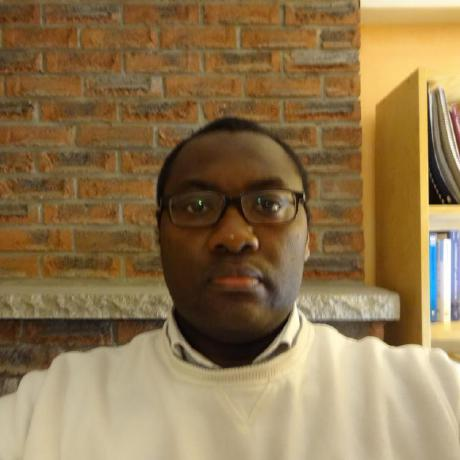
\includegraphics[scale=0.32]{../../francais/images/XavierNOUNDOU-2}
\captionof{figure}{Portrait of PR. XAVIER.\label{fig:xaviernoumbis}}
\end{center}

\textbf{\myfullacademicname} is a CHRISTIAN BY FAITH,
Cameroonian, born on September~$16$ $1983$ in
DOUALA (LITTORAL region, CAMEROON).

Xavier has a \textit{''Diplom--Informatiker (Dipl.--Inf.)''}
qualification from the \textbf{\unibremen, Bremen, Bremen, GERMANY} (May~$25$, $2007$).

Xavier is a \textit{PH.D. in Software Engineering}
(software construction, and testing) since November~$18$,~$2020$
because of his academic research, and professional engineering
contributions as follows:


\begin{enumerate}
%	\itemsep -0.7em
	\item 'Context-Sensitive Staged Static Taint Analysis
			For C using LLVM'
		\begin{enumerate}[1.]
			\itemsep -0.7em
			\item source code: \\
			\url{http://github.com/xnoumbissinoundou/yeroth-saint}
			\item full text (published on July~$1^\text{st}$, $2015$): \url{http://archive.org/details/saint_201507}.
		\end{enumerate}		 

	\item 'YEROTH-ERP-3.0':
			\begin{enumerate}[1.]
			\itemsep -0.7em
			\item source code: \\
			\url{http://github.com/xnoumbissinoundou/yeroth-erp-3.0}
			\item full text (ongoing publication): \url{http://archive.org/details/yeroth-erp-3-0-info-english}.
		\end{enumerate}	
\end{enumerate}


\vspace{-1.5em}
\section{Introduction}
\vspace{-0.3em}
\yeren is an \textbf{Enterprise Resource Planing} (ERP)
software--system. 

Users of \yeren could have the following roles:
\begin{enumerate}[1)]
	\itemsep -0.6em
	\item \administrator
	\item \manager
	\item \seller
	\item \inventorystockmanager
	\item \storekeeper
	\item \cashier.	
\end{enumerate}

\yeren allows for business management tasks 
listed in Table~\ref{tachesEtFonctions},
depending on user role.
\begin{table*}[!htbp]
\centering
\begin{tabular}{lccccc}
\centering \textbf{Tasks} 		& \managerb 		& \sellerb				& \inventorystockmanagerb 	& \storekeeperb	&	\cashierb 		 		\\ \hline
insert stock 					& \mycheckmark{blue}	&		& \mycheckmark{blue}	& 	&  				 			\\ \hline
delete stock 					& \mycheckmark{blue}	&		& 						&   &  							\\ \hline
view merchandise list			& \mycheckmark{blue}	& \mycheckmark{blue} & \mycheckmark{blue} & 				& 	\\ \hline
view stock 						& \mycheckmark{blue}	& \mycheckmark{blue} & \mycheckmark{blue} & \mycheckmark{blue}	& \mycheckmark{blue} 	\\ \hline
modify stock 					& \mycheckmark{blue}	&	& \mycheckmark{blue}		& 		&  				 			\\ \hline
transfer stock					& \mycheckmark{blue}	&	& \mycheckmark{blue}		& \mycheckmark{blue}	&  			\\ \hline
modify stock 					&  			& 			& 	& 					&	 								\\ 
management strategy  			& \mycheckmark{blue} 	& \mytimespartial{blue}	& \mytimespartial{blue}	& 	&  		\\ 
(ex.: \fifo, etc.)				&				 		&		&				&						&					\\ \hline
point--of--sale 		& \mycheckmark{blue}	& \mycheckmark{blue}	&						& 	& \mycheckmark{blue} 			\\ \hline
view stock transfers 		 	& \mycheckmark{blue}	&						& \mycheckmark{blue}	& \mycheckmark{blue}	&  							\\ \hline
stock buying management			& \mycheckmark{blue}	& \mytimespartial{blue}	& \mycheckmark{blue}	& 					& 	\\ \hline
customer management 			& \mycheckmark{blue}	& \mycheckmark{blue}	& 						& 					&  	\\ \hline
business dashboard 				& \mycheckmark{blue}	& 	&					& 					& \\\hline
view sales information 			& \mycheckmark{blue}	& \mytimespartial{blue}	&						& 					& 	\\ 	 				
\end{tabular}
\caption{\yerenpos functions--tasks, and associated users--roles.}\label{tachesEtFonctions}
\end{table*}

\begin{figure}[!htbp]
\centering
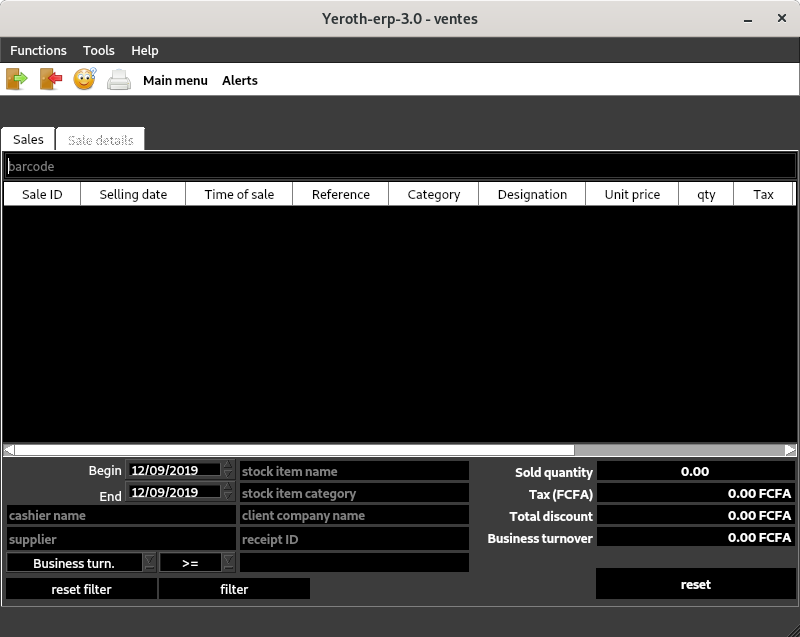
\includegraphics[scale=0.32]{../../francais/images/yeren-window-sale-information.png}
\caption{Sale--information window}
\label{fig:fenetre-de-la-vente}
\end{figure}

\vspace{-1.9em}
\section{Advantages of \yeren}
\vspace{-0.3em}
\begin{enumerate}[1)]
	\itemsep -0.3em
	\item \yeren is $100\%$ stable
	\item \yeren has an alert system with two types of alerts:
	      alerts based on stock--quantity, and time--period alerts
	\item users have the choice between small size receipts,
	      and, bigger size receipts (''A4'')
	\item \yeren runs on the Linux operating system,
	      because Linux is stable, performant, and less
	      vulnerable to security breaches in comparison
	      to other operating systems
	\item \yeren has an user interface ''Sales'', which
	      helps the \manager to view sales
	      information~(Figure~\ref{fig:fenetre-de-la-vente})
	\item \yeren has an interface ''Business--Dashboard'' that
		  generates pie and bar charts, from sales information,
		  in PDF format, to help the \manager to take
		  business--decisions.
\end{enumerate}

\vspace{-1.2em}
\section{Alert System}
\vspace{-0.3em}
\yeren allows users to create two types of alerts:
\begin{enumerate}[1)]
	\itemsep -0.5em
  \item alerts over stocks--quantities
  \item alerts over time intervals (this helps for
	  perissable articles and for sales discounts
	  over a period of time).
\end{enumerate}

\vspace{-1.1em}
\subsection{Alerts over Stock--Quantity}
\vspace{0em}
Users with the roles \administrator or \manager
could create alerts that will be triggered
whenever a ''pre--determined'' stock--quantity
will be reached.

For instance, Xavier (\manager) could create
an alert for stock ''mango'' that will be
trigerred whenever stock ''mango'' quantity
reaches $100$; this alert will be sent,
together with a message to user John (\storekeeper).

\vspace{-1.1em}
\subsection{Alerts over Time--Period}
\vspace{0em}
Users with roles \administrator or \manager
could create alerts that will be triggered
whenever a ''pre--specified'' ''gregorian''
calendar date will be reached.

For example, an alert with a message has to be
sent to Paul (\cashier) when the date of November
$18^{th}$ is reached. The alert's message
specifies that a rebate of $20\%$ has to be applied
on every sale of the yoghourt 'tr\`esbon', during a
time interval of $2$ weeks.

\vspace{-1.5em}
\section{Database Management System}
\vspace{-0.9em}
\yeren uses \emph{MySQL} as the standard DBMS. 
\emph{MySQL} is very stable, performant, and
free.

\vspace{-1.1em}
\section{Tasks of the User--Role \administrator}\label{tachesadmin}
\vspace{-0.3em}
The main tasks of a user with the role \administrator
among others are to:\\
\{\emph{create, modifiy, list, delete}\} $\longrightarrow$
\hspace{0.09cm} \{an alert, a category of articles,
a user account, a supplier account, a localisation\}.

\vspace{-0.5em}
\section{Conclusion}
\vspace{-0.9em}
\begin{figure}[!htbp]
\centering
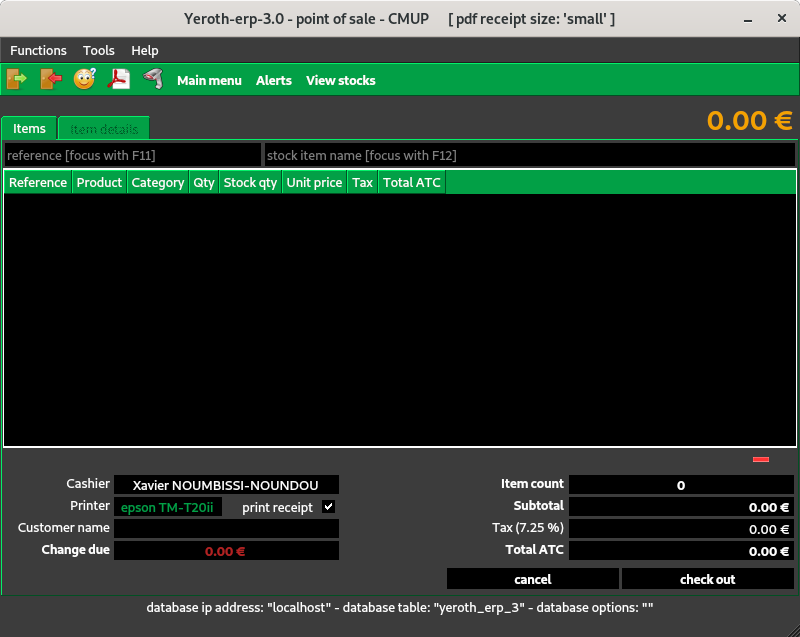
\includegraphics[scale=0.33]{../../francais/images/yeren-pos-7-0-window-cashier.png}
\caption{User--window to checkout articles--stocks.}
\label{fig:fenetre-de-vente}
\end{figure}

Figure~\ref{fig:fenetre-de-vente} illustrates the window
for selling articles.

\yeren is available in the English and French languages.

\end{document}
